\documentclass[a4paper,12pt]{article}

\newcommand{\me}{Jonathan R.\ J.\ Yong}
\newcommand{\meshort}{J.R.J.Y.}
\newcommand{\eriks}{{\=E}riks Kup{\v{c}}e}
\newcommand{\tim}{Tim D. W. Claridge}

% Fonts {{{1
\usepackage{fontspec,amsmath,unicode-math}
\setmainfont[
  Path={./fonts/},
  Extension=.otf,
  UprightFont={*-regular},
  BoldFont={*-semibold},
  ItalicFont={*-italic},
  BoldItalicFont={*-semibolditalic},
  Ligatures=TeX,
]{minion3}
\setmonofont[
  Path={./fonts/},
  Extension=.ttf,
  UprightFont={*-Regular},
  BoldFont={*-SemiBold},
  ItalicFont={*-Italic},
  BoldItalicFont={*-SemiBoldItalic},
  Scale=MatchLowercase
]{RobotoMono}
\setmathfont[
  Path={./fonts/},
  Scale=MatchLowercase
]{MinionMath-Regular.otf}
% Other optical sizes for Minion
\newfontfamily{\fontcaption}{minion3caption}[
  Path={./fonts/},
  Extension=.otf,
  UprightFont={*-regular},
  BoldFont={*-semibold},
  ItalicFont={*-italic},
  BoldItalicFont={*-semibolditalic},
  Ligatures=TeX,
]
\newfontfamily{\fontsubhead}{minion3subhead}[
  Path={./fonts/},
  Extension=.otf,
  UprightFont={*-regular},
  BoldFont={*-bold},
  ItalicFont={*-italic},
  BoldItalicFont={*-bolditalic},
  Ligatures=TeX,
]
\usepackage[final]{microtype}
% }}}1
% Packages and settings {{{1
\usepackage[font=small,labelfont=it,margin=15pt,skip=5pt]{caption}
\usepackage{fullpage,parskip,graphicx,float,braket,setspace,subcaption,booktabs}
\usepackage[svgnames]{xcolor}

% \usepackage{minted}
% \usepackage{tcolorbox}
% \tcbuselibrary{minted}
% \renewcommand{\MintedPygmentize}{./pygmentize_bruker.py}
% \usepackage{listings}
% \lstset{upquote=true}
% \newtcblisting{tcbminted}[1]{%
%     colframe=black,%
%     colback=white,%
%     width=0.95\textwidth,%
%     center,%
%     listing only,%
%     minted options={curlyquotes=false,fontsize=\small},%
%     minted language={#1},%
% }

\usepackage{chemformula}
\setchemformula{math-scripts=true}
\usepackage[style=chem-acs,subentry,articletitle,doi]{biblatex}
\addbibresource{hcosy.bib}
\graphicspath{{./figures/}}
\usepackage{xurl}   % must be after biblatex
\usepackage[
  mode=match,
  range-phrase={--},
  range-units=single,
  propagate-math-font=true,
  reset-math-version=false,
  reset-text-family=false,
  reset-text-series=false,
  text-family-to-math=true,
  text-series-to-math=true
]{siunitx}
\usepackage[symbol]{footmisc}
\usepackage{titletoc}
\usepackage{hyperref}
\hypersetup{
    naturalnames,
    colorlinks,
    linkcolor={black},
    citecolor={blue!60!black},
    urlcolor={blue!80!black}
}
\usepackage[capitalise,noabbrev]{cleveref}
\usepackage{usebib}
\newbibfield{entryset}
\bibinput{hcosy}
\onehalfspacing
\DeclareSIUnit{\molar}{\textsc{m}}
\DeclareSIUnit{\ppm}{ppm}
% }}}1
% Newcommands {{{1 
\DeclareMathOperator*{\sgn}{sgn}
\newcommand{\articletitle}{TITLE TO GO HERE}
\newcommand{\crl}{Chemistry Research Laboratory, Department of Chemistry, University of Oxford, Mansfield Road, Oxford OX1 3TA, United Kingdom}
\newcommand{\turing}{The Alan Turing Institute, The British Library, 96 Euston Road, London NW1 2DB, United Kingdom}
\newcommand{\brukeruk}{Bruker UK Ltd, R\&D, Coventry CV4 9GH, United Kingdom}
\newcommand{\exscientia}{Exscientia Ltd, The Schr{\"o}dinger Building, Oxford Science Park, Oxford OX4 4GE, United Kingdom}
\newcommand{\proton}{\ch{^{1}H}}
\newcommand{\carbonbulk}{\ch{^{12}C}}
\newcommand{\carbon}{\ch{^{13}C}}
\newcommand{\nitrogen}{\ch{^{15}N}}
\newcommand{\SInf}{\textit{Supplementary Information}}
\newcommand{\CH}{\carbon{}--\proton{}}
\newcommand{\HC}{\proton{}--\carbon{}}
\newcommand{\NH}{\nitrogen{}--\proton{}}
\newcommand{\HN}{\proton{}--\nitrogen{}}
\newcommand{\HH}{\proton{}--\proton{}}
\newcommand{\magn}[1]{\ch{^1H}$^{#1}$}
\newcommand{\magnnot}[1]{\ch{^1H}$^{!#1}$}
\newcommand{\todo}[1]{{\color{OrangeRed}#1}}
\newcommand{\changed}[1]{{\color{DodgerBlue!75!blue}#1}}
\newcommand{\autociteset}[1]{\autocite{\usebibentry{#1}{entryset}}}
\newcommand{\onejch}{{}^1\!J_{\ch{CH}}}
\newcommand{\onejcc}{{}^1\!J_{\ch{CC}}}
\newcommand{\onejnh}{{}^1\!J_{\ch{NH}}}
\newcommand{\onejxh}{{}^1\!J_{\ch{XH}}}
\newcommand{\njch}{{}^n\!J_{\ch{CH}}}
\newcommand{\njcc}{{}^n\!J_{\ch{CC}}}
\newcommand{\njnh}{{}^n\!J_{\ch{NH}}}
\newcommand{\njxh}{{}^n\!J_{\ch{XH}}}
\newcommand{\theurl}{\url{https://nmr-genesis.co.uk}}
\newcommand*{\brucine}{Spectra were obtained on a \SI{700}{\MHz} Bruker AV III equipped with a TCI H/C/N cryoprobe; the sample used was \SI{50}{\milli\molar} brucine in \ch{CDCl3}}
\newcommand*{\cyclo}{Spectra were obtained on a \SI{700}{\MHz} Bruker AV III equipped with a TCI H/C/N cryoprobe; the sample used was \SI{50}{\milli\molar} cyclosporin A in \ch{C6D6}}
\newcommand{\angang}[2]{#1\rlap{\unit{\degree}}\ensuremath{_{#2}}}
% }}}1
% NOAH macros {{{1
\newcommand{\abn}{NOAH-2 AB$_{\ch{N}}$}
\newcommand{\abnbn}{NOAH-3 A(B$_{\ch{N}}$/B$_{\ch{N}}$)}
\newcommand{\abnbs}{NOAH-4 A(B$_{\ch{N}}$/B/S)}
\newcommand{\abnns}{NOAH-4 A(B$_{\ch{N}}$/N/S)}
\newcommand{\abnbspns}{NOAH-5 A(B$_{\ch{N}}$/B/S$^{+}_{\ch{N}}$/S)}
\ExplSyntaxOn
\msg_new:nnn{noah}{module-not-found}{Module~code~`#1'~not~recognised.~If~it~was~not~a~typo,~you~may~need~to~define~this~in~\c_backslash_str noahmodule.}
\NewDocumentCommand{\noahmodule}{m}{
    \str_case:nnTF{#1}{
        {A}{A}
        {Bn}{B${}\sb{\ch{N}}$}
        {B}{B}
        {Cc}{C$\sp{\text{c}}$}
        {Cqf}{C$\sp{\text{qf}}$}
        {C}{C}
        {D}{C}
        {Jqf}{J$\sp{\text{qf}}$}
        {J}{J}
        {Mn}{M$\sb{\ch{N}}$}
        {M}{M}
        {N}{N}
        {O}{O}
        {Pt}{P$\sp{\text{T}}$}
        {P}{P}
        {R}{R}
        {Sc}{S$\sp{\text{C}}$}
        {Sn}{S$\sb{\ch{N}}$}
        {Spa}{S$\sp+\sb1$}
        {Spb}{S$\sp+\sb2$}
        {Spn}{S$\sp{+}\sb{\ch{N}}$}
        {Sp}{S$\sp+$}
        {St}{S$\sp{\text{T}}$}
        {S}{S}
        {T}{T}
        {X}{X}
        }{}{\textbf{?}
        \msg_error:nnn{noah}{module-not-found}{#1}}
}
\NewDocumentCommand{\noah}{s m}{
    \IfBooleanTF{#1}{}{NOAH-\clist_count:n{#2}~}
    {\clist_map_inline:nn{#2}{\noahmodule{##1}}}
}
\ExplSyntaxOff
% }}}1

\begin{document} \begin{refsection}

\begin{center}   % Front matter
    \textbf{\Large \articletitle{}}

    \vspace{0.2cm}

    \me{},\textsuperscript{1} \eriks{},\textsuperscript{2} \tim\textsuperscript{1,\texttt{*}}

    \vspace{0.2cm}

    \small

    \textsuperscript{1} \textit{\crl{}}

    % \textsuperscript{2} \textit{\turing{}}

    \textsuperscript{2} \textit{\brukeruk{}}

    % \textsuperscript{4} \textit{\exscientia{}}

    \normalsize \textsuperscript{\texttt{*}} \texttt{tim.claridge@chem.ox.ac.uk}

    \vspace{0.5cm} \hrule

\end{center}

\section*{Abstract}
\begin{figure*}[ht]
    \centering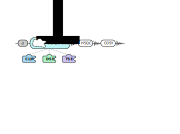
\includegraphics{toc.png}%
\end{figure*}

BLAH

\section{Introduction}

\section{Conclusion}


\section*{Acknowledgements}

We thank Dr Mohammadali Foroozandeh (University of Oxford) for helpful discussions.
\meshort{}\ thanks the Clarendon Fund (University of Oxford) and the EPSRC Centre for Doctoral Training in Synthesis for Biology and Medicine (EP/L015838/1) for a studentship, generously supported by AstraZeneca, Diamond Light Source, Defence Science and Technology Laboratory, Evotec, GlaxoSmithKline, Janssen, Novartis, Pfizer, Syngenta, Takeda, UCB, and Vertex.

% Fakesection Bibliography
\AtNextBibliography{\small}
\printbibliography{}
\end{refsection}


% Fakesection ================= SI ==================

\clearpage
\begin{refsection}
\newcommand{\sectionbreak}{\clearpage}
\renewcommand*{\thefigure}{S\arabic{figure}}
\renewcommand*{\thesection}{S\arabic{section}}
\renewcommand*{\thetable}{S\arabic{table}}
\renewcommand*{\thepage}{S\arabic{page}}
\setcounter{page}{1}
\setcounter{figure}{0}
\setcounter{section}{0}
\setcounter{table}{0}
\onehalfspacing

\hspace{0pt}
\vfill
\begin{center}
    \huge
    Supporting Information

    \vspace{0.3cm}

    \textit{for}

    \vspace{0.3cm}

    \articletitle{}

    \vspace{0.6cm}

    \Large \me{},\textsuperscript{1} \eriks{},\textsuperscript{2} \tim{}\textsuperscript{1,\texttt{*}}

    \vspace{0.6cm}

    \large \textsuperscript{1} \textit{\crl{}}

    \textsuperscript{2} \textit{\brukeruk{}}

    \textsuperscript{\texttt{*}} \texttt{tim.claridge@chem.ox.ac.uk}

\end{center}
\vfill

\newpage
\section*{Contents}

\startcontents[si]
\printcontents[si]{ }{1}{}
\vfill
\hspace{0pt}
\newpage

\section{Software and raw data}

All processing was carried out using TopSpin 3 or 4.
Plots are generated in Python 3, using the \href{https://github.com/numpy/numpy}{\texttt{numpy}}, \href{https://github.com/scipy/scipy}{\texttt{scipy}}, and \href{https://github.com/yongrenjie/penguins}{\texttt{penguins}} libraries.
The raw data used for this paper, as well as all scripts required for regenerating the plots, are available on GitHub: \url{https://github.com/yongrenjie/hsqc-cosy-paper}.

% Fakesection SI bibliography
\AtNextBibliography{\small}
\printbibliography{}
\clearpage    % For some reason this is needed to make the last page number 'S5', not '5'

\end{refsection}

\end{document}
